\chapter{Basic iterative methods}%
\label{cha:Basic iterative methods}

We want to solve the linear system
\[
	Au = f \qquad (Ax = h)
.\] 
\begin{itemize}
	\item traditional directl methodes (Gauss elemination) are insufficient:
		\begin{itemize}
			\item $\O(n^{4})$ steps
			\item $\O(n^{3})$ storage units
		\end{itemize}

	\item Iterative methods try to improve an implicit guess until some tolerance criterion is reached
		\begin{itemize}
			\item $\O(n^{2})$ storage units
		\end{itemize}
\end{itemize}

\section{Relaxation methods}%
\label{sec:Relaxation methods}

Basic relaxation methods are based on a coordinate-wise relaxation/reduction of an initial residuum
\[
\gamma = b- Ax
.\] 
In each relaxation step these methodes try to annihilate a component of the residual.

The general idea is to transform the linear system into a fixed point problem
\[
	x = x + P^{-1}(b-Ax)
,\] 
where $P$ is called a proconditioner (matrix) and should be easy to invert in the sense that $Pe=r$ can be solved easily and $P$ should be an approximation of matrix $A$.

Basic idea to solve a fixed-point problem is a fixed-point iteration
\[
	x^{k+1} = x^{k} + P^{-1}(b-Ax^{k})
.\] 
Rewriting this to make it a bit prettier results in
\[
	x^{k+1} = Gx^{k} + g =:T(x^{k})
.\] 
where $G = I-P^{-1}A$ is the iteration matrix and $g = P^{-1}b$.

\subsection{Some examples of relaxation schemes}
\label{sec:Some examples of relaxation schemes}

\begin{enumerate}[label=\Alph{enumi})]
	\item Jacobi method 

		Let $P_{J} = \diag(A)$, then obviously
		\[
			x^{k+1} = x^{k} + \diag(A)^{-1}(b-Ax^{k})
		.\] 
		written in terms of the components
		\[
			x^{k}= (\xi _{i}^{k})_{i}, \quad b=(\beta_{i})_{i}
		\] 
		gives
		\[
			a_{ii}\xi _{i}^{(k+1)} = -\sum_{\substack{j=1 \\ j \neq i}}^{n}{a_{ij}\xi _{j}^{(k)}+ \beta_{i}}
		.\] 
		Let $A=D-L-U$ be a splitting of the matrix $A$ into diagonal $D$, lower triangular part $L$ and upper triangular part $U$
		\[
		A = \begin{pmatrix}
			\diagdown & & -U \\
			  &D&    \\
			-L & & \diagdown
		\end{pmatrix}
		.\] 
		Then $P_{J} = D$
		\[
			Dx^{k+1} = (L+U)x^{k} + b
		.\] 
		For the 5-point stencil $\laplace_{h}^{(5)}$ we have 
		\[
			D = \diag(\frac{4}{h^{2}}) 		
		\] 
		and the matrix $L+U$ looks like the following image.
		\begin{figure}[H]
			\begin{center}
				\includegraphics[width=0.5\textwidth]{pics/chapter1/huebschematrix.png}
			\end{center}
			\caption{$L+U$}
			\label{fig:huebschematrix}
		\end{figure}
		
		So written directly in terms of the grid vector $u_{i,j}$ we get the Jacobi scheme for inner nodes
		\[
			u_{i,j}^{k+1} = \frac{1}{4}(u_{i,j-1}^{k}+ u_{i-1,j}^{k} + u_{i,j+1}^{k} + u_{i+1,j}^{k} + h^{2}f_{i,j})
		.\] 
		\underline{Note}: Instead of $P=D$ one could implement a \underline{damped Jacobi scheme} with
		\[
			P_{J}(\omega )=\omega \cdot D \qquad \text{ with } 0 < \omega \leq 1
		.\] 
	\item Gauss-Seidel Relaxation

		Instead of diagonal $P$, we use triangular matrix
		\[
			\underset{\text{ (forward) }}{P_{GS} = D-L} \quad\text{ or }\quad \underset{\text{ (backward) }}{P_{GS'}=D-U}
		.\] 
		\begin{figure}[H]
			\begin{center}
				

\tikzset{every picture/.style={line width=0.75pt}} %set default line width to 0.75pt        

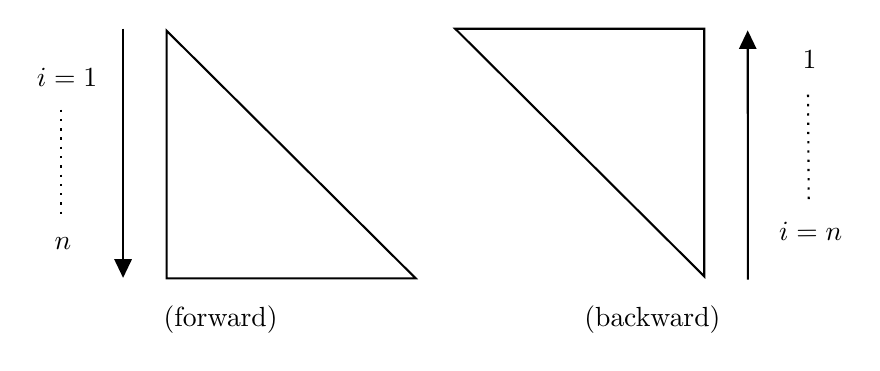
\begin{tikzpicture}[x=0.75pt,y=0.75pt,yscale=-1,xscale=1]
%uncomment if require: \path (0,170); %set diagram left start at 0, and has height of 170

%Shape: Right Triangle [id:dp5671683907330274] 
\draw   (201,11.71) -- (321,131) -- (201,131) -- cycle ;
%Straight Lines [id:da39919664072609184] 
\draw    (180,10.71) -- (180,128.71) ;
\draw [shift={(180,130.71)}, rotate = 270] [fill={rgb, 255:red, 0; green, 0; blue, 0 }  ][line width=0.75]  [draw opacity=0] (8.93,-4.29) -- (0,0) -- (8.93,4.29) -- cycle    ;

%Straight Lines [id:da8365689488016284] 
\draw  [dash pattern={on 0.84pt off 2.51pt}]  (150,49.71) -- (150,100.71) ;



%Shape: Right Triangle [id:dp24623033400831917] 
\draw   (460,130) -- (340,10.71) -- (460,10.71) -- cycle ;
%Straight Lines [id:da8106199446608251] 
\draw    (481.05,131.54) -- (480.95,13.54) ;
\draw [shift={(480.95,11.54)}, rotate = 449.95] [fill={rgb, 255:red, 0; green, 0; blue, 0 }  ][line width=0.75]  [draw opacity=0] (8.93,-4.29) -- (0,0) -- (8.93,4.29) -- cycle    ;

%Straight Lines [id:da46079427117101157] 
\draw  [dash pattern={on 0.84pt off 2.51pt}]  (510.34,92.76) -- (510,41.71) ;





% Text Node
\draw (153,34) node   {$i=1$};
% Text Node
\draw (151,114) node   {$n$};
% Text Node
\draw (511.22,108.46) node [rotate=-359.54]  {$i=n$};
% Text Node
\draw (510.82,25.47) node [rotate=-0.41]  {$1$};
% Text Node
\draw (227,151) node  [align=left] {(forward)};
% Text Node
\draw (435,151) node  [align=left] {(backward)};


\end{tikzpicture}

			\end{center}
			\caption{forward and backward iteration matrix form}
			\label{fig:forwardbackward}
		\end{figure}
		
		We get the component-wise scheme
		\[
			\xi _{i}^{(k+1)}=\frac{1}{a_{ii}} \Big( -\sum_{j=1}^{i-1}{a_{ij}} \xi _{j}^{(k+1)}-\sum_{j=i+1}^{n}{a_{ij}\xi _{j}^{k}} + \beta _{i} \Big) \qquad i=1, \ldots, n
		\] 
		or (backward)
		\[
			\xi _{i}^{(k+1)} = \frac{1}{a_{ii}} \Big( -\sum_{j=1}^{i-1}{a_{ij}\xi _{i}^{(k)}}-\sum_{j=i+1}^{n}{a_{ij}\xi _{j}^{(k+1)}} + \beta _{i} \Big) \qquad i=n, \ldots ,1
		.\] 
		\underline{Note} : A damped relaxation method uses:
		\[
			P_{GS}(\omega ) := \frac{1}{\omega }(D-L) \quad \text{ or } \quad P_{GS'}(\omega ) := \frac{1}{\omega }(D-U)
		\] 
		i.e. (forward)
		\[
			\xi _{i}^{(k+1)} = (1-\omega )\xi _{i}^{(k)} + \frac{\omega }{a_{ii}} \Big( -\sum_{j=1}^{i-1}{a_{ij}\xi _{j}^{(k+1)}} - \sum_{j=i+1}^{n}{a_{ij}\xi _{j}^{(k)}} + \beta _{i} \Big) 
		.\] 
	\item Richardson relaxation
		\begin{align*}
			P_{R}(\omega ) :&= \frac{1}{\omega } I \\
			\xi _{i}^{(k+1)} &= \xi _{i}^{(k)} + \omega \Big( -\sum_{j=1}^{n}{a_{ij}\xi _{j}^{(k)}} + \beta _{i} \Big) 
		\end{align*}
\end{enumerate}
		Questions:
		\begin{itemize}
			\item How to characterize convergence?
			\item How to choose the relaxation parameter $\omega $?
		\end{itemize}

		Denote by $e^{k} := A^{-1}b - x^{k}$ the error in the k-th iteration and by $G:=I-P^{-1}A$ the iteration matrix. So
		\[
			e^{k+1}= (I-P^{-1}A)e^{k} = Ge^{k} = G^{2}e^{k-1} = \cdots = G^{k+1}e^{0}
		.\] 
		Taking the norm on both sides results in
		\[
			\norm{e^{k+1}}  \leq \normiii{(I-P^{-1}A)^{k+1}} \cdot \norm{e^{0}} 
		\] 
		with vector norm $\norm{\cdot}$ and induced matrix norm $\normiii{\cdot}$.
		\begin{lemma}
		\label{thm:richardconvergencelemma}
		The error norm $\norm{e^{k}} \rightarrow 0$ ( for $k \rightarrow \infty$) and $x^{k} \rightarrow A^{-1}b$ for all initial errors $e^{0}$ $\iff$
		\[
			\lim_{k \to \infty} \normiii{(I-P^{-1}A)^{k}} = 0
		.\] 
		The proof is omitted here and can be read in 
		[Greenbaum 97. Lemma 2.11].
		\end{lemma}

		\begin{theorem}
		\label{thm:richardconvergencetheorem}
			$x^{k} \rightarrow A^{-1}b$ for $k \rightarrow \infty$ for all initial values $x^{0}$ $\iff$
			\[
				\rho(I-P^{-1}A) < 1
			.\] 
			(with $\rho(\cdot)$ the spectral radius of the matrix)
		\end{theorem}
		\begin{proof}\
		\label{thm:richardconvergencetheoremproof}
		\begin{itemize}
			\item "$\Longrightarrow$" 

				Assume that $x^{k}\rightarrow A^{-1}b$ converges. 
				Let $\lambda $ be the eigenvalue of $G$ with $\abs{\lambda} = \rho(G)$ and $x$ be the associated eigenvector.
				
				Choose $b=0$ and $x^{0}=cx$ for any $c \in \R \setminus \left\{ 0 \right\} $. We get
				\[
				x^{k+1} = Gx^{k} = G^{k+1}x^{0} = \lambda ^{k+1} x^{0}
				.\] 
				\[
					\begin{array}{rl}
						\abs{\lambda } >1 &\implies \text{ divergence } \\
						\abs{\lambda }  = 1 &\implies \text{ no convergence }
				\end{array}
				\lightning
				.\] 
			\item "$\Longleftarrow$"

				Assume $\rho(G)<1$.

				There exists an $\epsilon >0$ and norm in $\R^{n \times n}$ such that.
				\[
					\normiii{G} \leq \rho(G) + \epsilon  < 1
				\] 
				with the previous lemma we get convergence.
		\end{itemize}
		[also see Y. Saad 03. Corollary 4.2]
		\end{proof}

\begin{definition}
\label{thm:additivesplitting}
Let $A, M, N$ be three given matrices with $ A = M-N$. The pair $(M,N)$ is called a \underline{regular splitting} of $A$ if
\begin{itemize}
	\item $M$ is non-singular
	\item $M^{-1}, N$ are non-negative (i.e. all entries are non-negative) ($M^{-1} \geq 0, N \geq 0$)
\end{itemize}
\end{definition}
With this splitting, the relaxation scheme can be written as 
\[
	x^{k+1} = \underbrace{M^{-1}N}_{G} x^{k} + M^{-1}b
.\] 
Thus
\begin{align*}
M \overset{\wedge}&{=} P \\
N \overset{\wedge}&{=} P-A
\end{align*}

\begin{theorem}
\label{thm:regularsplittingtheorem}
Let $M,N$ be a regular splitting of $A$. Then $\rho(\underbrace{M^{-1}N}_{G} ) < 1$ $\iff$

A is non-singular and $A^{-1}$ is non-negative.
\end{theorem}

\begin{proof}\
\label{thm:regularsplittingtheoremproof}
\begin{itemize}
	\item "$\Longrightarrow$"

		Assume $\rho(G) < 1$. 
		\[
			A = \underbrace{M}_{\text{ non-sing. }}\cdot \underbrace{(I-G)}_{\text{ non-sing. }} = M -MG = M-N
		.\] 
		So $A$ is non-singular as a product of non-singular matrices.
		\[
			(I-G)^{-1} = \sum_{i=0}^{\infty}{G^{i}}
		\] 
		with $G$ non-negative. So the powers $G^{i}$ are non-negative. Hence $(I-G)^{-1}$ is non-negative.
		\[
		\implies A^{-1} \text{ is non-negative. }
		.\] 
	\item "$\Longleftarrow$"

		Assume $A$ is non-singular and $A^{-1}$ is non-negative.

		Since $A$ and $M$ are non-singular, the matrix $(I-G)$ is non-singular.
		\begin{align*}
			A^{-1}N &= (M(I-M^{-1}N))^{-1}N \\
					&= (I-M^{-1}N)^{-1}M^{-1}N \\
					\tag{$\ast\ast$}
					&= (I-G)^{-1}G
		\end{align*}

		\[
		M^{-1}, N \geq 0 \qquad G = M^{-1}N \geq 0
		.\] 

		Let $\lambda $ be an eigenvalue of $G$ with $\abs{\lambda }=\rho(G)$ and associated eigenvector $x$ with $x \geq 0$ (Perron-Frobenius)
		\[
			Gx = \rho(G)x
		\] 
		and with $(\ast\ast)$ we get $A^{-1}Nx = (I-G)^{-1}x = \frac{\rho(G)}{1 - \rho(G)}x$.

		This implies
		\[
			\frac{\rho(G)}{1-\rho(G)} \geq 0
		\] 
		and so $0 \leq \rho(G) \leq 1$.

		Since $(I-G)$ is non-singular, $\rho(G) \neq 1$.

		[also see Y.Saad 03 Th.4.4]
\end{itemize}
\end{proof}

\begin{lemma}
\label{thm:matrixequivalences}
	Let $A \in \R^{n \times n}$ with $a_{ij} \leq 0, i \neq j$. Then the following statements are equivalent:
	\begin{enumerate}[label=\arabic{enumi})]
		\item $A$ is an M-matrix
		\item $A$ is non-singular and $A^{-1} \geq 0$ (and $a_{ii} > 0$)
		\item $a_{ii} > 0$ and $A\cdot D$ is strictly (row-) diagonally dominant for some diagonal matrix $D$
	\end{enumerate}
	
	For a proof see [Horn, Johnson : Topics of matrix analysis, 91']
\end{lemma}

\begin{theorem}
\label{thm:theorem2.3}
	If $A$ is strictly diagonally dominant or irreducibly diagonally dominant, then the associated Jacobi and GS iteration scheme converges for any initial vector $x^{0}$.
\end{theorem}

\begin{proof}
\label{thm:theorem2.3proof}
	[Y. Saad 03 Theorem 4.9]
\end{proof}

What is the "optimal" relaxation parameter?

In which sense "optimal"?

Denote by $G(\omega )=I-P^{-1}(\omega )A$ the iteration matrix induced by $P(\omega )$.

We say $\omega $ is optimal if
\[
	\omega  = \argmin_{\alpha \in \R^{+}} \rho(G(\alpha ))
.\] 
An iteration scheme is called \underline{underrelaxation method} if $\omega  < 1$. Otherwise it is called \underline{overrelaxation method}.

\begin{theorem}
\label{thm:theorem2.4}
Let $G_{J}$ be the iteration matrix of the Jacobi relaxation and assume	$G_{J}$ has only real eigenvalues $\lambda_1 \leq \lambda_2 \leq \ldots \leq \lambda_{n}$ with linear independent eigenvectors $x_1, \ldots , x_{n}$ and $\rho(G_{J}) < 1$. Then the iteration matrix $G_{J}(\omega )$ has eigenvalues
\[
\mu _{i} =  1 - \omega - \omega \lambda _{i}
\] 
and 
\[
\omega _{\text{opt}} = \frac{2}{2-\lambda_1-\lambda _{n}}
\] 

Proof can be found in [A. Meister Numerik linearer Gleichungssysteme]
\end{theorem}

\begin{figure}[H]
	\begin{center}
		

\tikzset{every picture/.style={line width=0.75pt}} %set default line width to 0.75pt        

\begin{tikzpicture}[x=0.75pt,y=0.75pt,yscale=-1,xscale=1]
%uncomment if require: \path (0,170.14285278320312); %set diagram left start at 0, and has height of 170.14285278320312

%Shape: Circle [id:dp48653499037477466] 
\draw  [color={rgb, 255:red, 80; green, 227; blue, 194 }  ,draw opacity=1 ][dash pattern={on 4.5pt off 4.5pt}] (270.14,85.86) .. controls (270.14,52.72) and (297.01,25.86) .. (330.14,25.86) .. controls (363.28,25.86) and (390.14,52.72) .. (390.14,85.86) .. controls (390.14,118.99) and (363.28,145.86) .. (330.14,145.86) .. controls (297.01,145.86) and (270.14,118.99) .. (270.14,85.86) -- cycle ;
%Straight Lines [id:da9383991483926752] 
\draw    (230,86.86) -- (430,86.86) (250,82.86) -- (250,90.86)(270,82.86) -- (270,90.86)(290,82.86) -- (290,90.86)(310,82.86) -- (310,90.86)(330,82.86) -- (330,90.86)(350,82.86) -- (350,90.86)(370,82.86) -- (370,90.86)(390,82.86) -- (390,90.86)(410,82.86) -- (410,90.86) ;


%Straight Lines [id:da8897299753707606] 
\draw  [dash pattern={on 0.84pt off 2.51pt}]  (330.14,5.86) -- (330.14,165.86) ;




% Text Node
\draw (273,103) node   {$\lambda _{1}$};
% Text Node
\draw (393,101) node   {$\lambda _{n}$};


\end{tikzpicture}
	\end{center}
	\caption{eigenvalues lie on opposite sites on the unit sphere}
	\label{fig:eigenwerte}
\end{figure}


\underline{Note}: So in case of symmetric eigenvalue around the origin we get $\omega _{\text{opt}}=1$

\begin{theorem}
\label{thm:theorem2.5}
	Let $A \in \R^{n \times n}$ with $a_{ii} \neq 0$
	\[
		\rho(G_{GS}(\omega )) \geq \abs{\omega -1} 
	.\] 
\end{theorem}

\begin{proof}
\label{thm:theorem2.5proof}
Let $\lambda _{1}, \ldots , \lambda _{n}$ be eigenvectors of $G_{GS}(\omega )$.
\begin{align*}
	\prod_{i=1}^{n} \lambda _{i} &= \det G_{GS}(\omega ) \\
								 &= \det ((D-\omega L)^{-1}) \det ((1+\omega ) D+ \omega U) \\
								 &= \det (D^{-1}) \det((1-\omega )D) \\
								 &= \det D^{-1} (1-\omega )^{n} \det D \\
								 &= (1-\omega )^{n}
\end{align*}

\end{proof}

\begin{mdframed}
	\underline{Remark}  : The script might miss some parts here due to an interactive reading course lecture experiment.

	For damped iteration schemes (Gauss-Seidel \& Richardson) we considered the questions:
	\begin{enumerate}[label=(\arabic{enumi})]
		\item For which $\omega $ do we get convergence?
		\item What is the spectral radius $\rho(G(\omega ))$?
		\item What is the optimal parameter choice $\omega _{\text{opt}}$?
		\item Requirements on the matrix $A$?
		\item How to choose $\omega $ iteratively?
	\end{enumerate}
	For answers look here:
	\begin{enumerate}[label=(\alph{enumi})]
		\item Gauss-Seidel / SOR (successive overrelaxation)
			\begin{itemize}
				\item Y. Saad, Ch. 4.2.5, Thm. 4.1.6
				\item A. Greenbaum, Ch. 10.11, Thm 10.1.3
				\item W. Hackbusch, Ch. 4.4.3
				\item A. Meister, Ch. 4.1.3.2
			\end{itemize}
		\item Richardson
			\begin{itemize}
				\item Y. Saad, Example 4.1
				\item W. Hackbusch, Ch. 4.4.1
				\item A. Meister, Ch. 4.1.4
			\end{itemize}
	\end{enumerate}
\end{mdframed}

\begin{mdframed}
%\label{thm:}
	\underline{Results for GS/SOR method}:

	\begin{thm}
	%\label{thm:}
		Let $A = I - L - U$ with
		\begin{equation}\label{eq:gsstar}\tag{$\ast$}
			\forall c \in \R ~ \forall\gamma  \in \R \setminus \left\{ 0 \right\}: \qquad \det(cI-L-U) = \det(cI-\gamma L - \gamma ^{-1}U) 
		\end{equation}
		and $\lambda \neq 0$ is eigenvalue of $G_{GS}(\omega )$ for $\omega \in(0,2)$, then
		\[
		\mu  = \frac{\lambda +\omega +1}{\omega \lambda ^{\frac{1}{2}}} \text{ is eigenvalue of }G_{J}
		.\] 
	\end{thm}
	\begin{thm}
	%\label{thm:}
		If
		\begin{itemize}
			\item $A$ satisfies \href{eq:gsstar}{($\ast$)} 
			\item $G_{J}$ only real eigenvalues
			\item $\beta = \rho (G_{J}) < 1$
		\end{itemize}
		Then
		\begin{itemize}
			\item SOR converges
			\item \[
					\rho (G_{GS}(\omega )) = \begin{cases}
						\frac{1}{4} \left[ \omega \beta + \sqrt{(\omega \beta )^2 + 4(\omega +1)}  \right]^2 & \text{ for }0 < \omega \leq \omega _{opt} \\
						\omega -1 & \text{ for } \omega _{opt} \leq  \omega < 2
					\end{cases}
			.\] 
		\item $\omega _{opt} = \frac{2}{1 +\sqrt{1-\beta ^2} }$
		\end{itemize}
	\end{thm}

	\underline{Results for Richardson method} : N/A
\end{mdframed}

\section{Symmetric splitting schemes}
\label{sec:Symmetric splitting schemes}

Let $P$
\begin{itemize}
	\item easy to invert
	\item approx. $A$
\end{itemize}
If $P$ is symmetric and positive definite, we could rewrite our linear system as:
\[
	\left.
	\begin{array}{rl}
	\underbrace{P^{-\frac{1}{2}}A P^{-\frac{1}{2}}}_{\tilde{A}} y &= \underbrace{ P^{-\frac{1}{2}}b}_{\tilde{b}} \\
	P^{-\frac{1}{2}}y &= x
	\end{array}
	\right\}
	\tilde{A} y = \tilde{b}
.\] 
If A ist positive definite then $\tilde{A}$ is also positive definite. This procedure is called "(symmetric) preconditioning" of $Ax = b$.

We have
\begin{itemize}
	\item Jacobi preconditioner $P_{J}$ is symmetric and for $\omega , d_{ii} \in \R_{>0}$ also positive definite.
	\item Richardson preconditioner $P_{R}$ is symmetric and positive definite for $\omega \in \R_{>0}$.
	\item Gauss-Seidel preconditioner $P_{GS}(\omega )$ is not symmetric.
\end{itemize}

\underline{How to symmetrize GS?} 

We try to combine forward and backward GS
	\begin{align*}
		(\omega ^{-1}D-L) x^{k+\frac{1}{2}} &= b -\left( \frac{\omega -1}{\omega }D-U \right) x^{k} \\
		(w^{-1}D-U) x^{k+1} &= b- \left( \frac{\omega -1}{\omega }D-L \right) x^{k+\frac{1}{2}} \\
							&= b - \left( \frac{\omega -1}{\omega }D-L \right) (\omega ^{-1}D-L)^{-1}\Big(b-\left(\frac{\omega -1}{\omega }D-U\right)x^{k}\Big)
	\end{align*}
	It follows
	\[
	x^{k+1}=Gx^{k} + P^{-1}b
	\] 
	with
	\begin{align*}
		G &= (D-\omega U)^{-1} \Big( (1-\omega )D+\omega L)\Big)(D-\omega L)^{-1} \Big( (1-\omega ) D + \omega U \Big) \\
		P^{-1}&= \omega (2-\omega )(D-\omega U)^{-1}D (D-\omega L)^{-1}
	\end{align*}
	\[
\implies P \text{ symmetric positive definite }	
	.\] 
	\[
		\implies \text{ scheme is called symmetric SOR \underline{(SSOR)} } (\text{ if } \omega > 1)
	.\] 

\section{Block-relaxation methods}%
\label{sec:Block-relaxation methods}

Instead of eliminating individual components of the residual, we could work with blocks of components:

Let
\[
A = \begin{bmatrix}
\begin{bmatrix}
A_{11}
\end{bmatrix}
&\cdots & 
\begin{bmatrix}
A_{1p}
\end{bmatrix} \\
\vdots &\ddots& \vdots\\
\begin{bmatrix}
A_{p1}
\end{bmatrix}
&\cdots & 
\begin{bmatrix}
A_{pp}
\end{bmatrix}
\end{bmatrix}
\qquad
x = \begin{bmatrix}
x_1 \\ \vdots \\ x_{p}
\end{bmatrix}
\qquad
b = \begin{bmatrix}
b_1 \\ \vdots \\ b_{p}
\end{bmatrix}
.\] 
One block of a matrix-vector product $Ax$:
\[
	(Ax)_{i} =  \sum_{j=1}^{p}{A_{ij}x_{j}}
.\] 
Analogously to the point-relaxation schemes, we introduce a splitting $A = D-L-U$ with
\[
D=
\begin{bmatrix}
	\begin{bmatrix}
	A_{11}
	\end{bmatrix}
	\\
	&\begin{bmatrix}
	A_{22}
	\end{bmatrix}
	\\
	&&\ddots
	\\
	&&&\begin{bmatrix}
	A_{pp}
	\end{bmatrix}
\end{bmatrix}
\qquad
L = \begin{bmatrix}
0 \\
\begin{bmatrix}
	A_{21}
\end{bmatrix}
& 0 \\
&\begin{bmatrix}
A_{32}
\end{bmatrix}
\\
&&\ddots \\
&&&\begin{bmatrix}
A_{p p-1}
\end{bmatrix}
& 0
\end{bmatrix}
\] 
and $U=D-L-A$.

Thus for the Jacobi method, we get the scheme
\[
	A_{ii}x_{i}^{(k+1)} = b_{i}+\Big( (L+U)x^{k} \Big) _{i} = b_{i} - \sum_{j \neq i}^{}{A_{ij}x_{j}^{(k)}}
.\] 
Typically $A_{ii}$ are much smaller than $A$ and sometimes simple to invert.
\begin{exam}
%\label{thm:}
	Finite Differences $A=\laplace_{h}^{(5)}$ with lexicographical ordering:
	\[
	A_{ii} = A_{0} = \frac{1}{h^2}\begin{bmatrix}
		4 & -1 \\
		-1 & 4 \\
		&&\ddots \\
		&&&4& -1\\
		&&&-1 & 4
	\end{bmatrix}
	\in \R^{(N_{x}+2) \times (N_{x} +2)}
	.\] 
	This matrix is tridiagonal.
	\[
	L+U = \frac{1}{h^2}\begin{bmatrix}
	& I \\
	I && \ddots \\
  	&\ddots &&I \\
	&&I
	\end{bmatrix}
	.\] 
	with $n_1 = n_2 = \ldots  N_{x} +2$ and $p=N_{y}+2$

	\begin{itemize}
		\item efficient Algorithm: Thomas Algorithm
		\item all blocks are the same
		\item factorize only once
	\end{itemize}
\end{exam}

\subsection{General block concept}
\label{sec:General block concept}

\underline{Basic iteration}

Let $S=\left\{ 1, \ldots, n \right\} $ be the overall index set. Partition $S$ into subsets $S_{i}$ ($i=1, \ldots, p$) (not necessarily disjunct) with
\[
S_{i}\subseteq S \qquad \bigcup_{i=1, \ldots, p}S_{i} = S
.\] 
If $S_{i}\cap S_{j} = \emptyset$ ($i \neq j$) we call this a \underline{non-overlapping} partitioning of $S$, otherwise a \underline{overlapping} partitioning.\enter

In the following let $n_{i}= \abs{S_{i}} $ be the size of the subset $S_{i}$ and 
\[
S_{i}= \left\{ m_{i}(1), m_{i}(2), \ldots , m_{i}(n_{i}) \right\} 
.\] 

To restrict the rows/columns of a matrix to the subsets, we use a transformation matrix
\[
	V_{i}= \left[ e_{m_{i}(1)}, e_{m_{i}(2)}, \ldots , e_{m_{i}(n_{i})} \right] \in \R^{n \times n_{i}}
.\] 
Additionally we introduce the matrices $W_{i} \in \R^{n \times n}$ such that
\[
\sum_{i=1}^{p}{V_{i}W_{i}^{T}} = I \in \R^{n \times n}
.\] 
Therefor choose $\eta _{m_{i}(j)} \in \R$ such that
\[
	W_{i} = \left[ \eta _{m_{i}(1)}e_{m_{i}(1)}, \ldots , \eta _{m_{i}(n_{i})}e_{m_{i}(n_{i})} \right] 
,\] 
e.g.
\[
\eta _{i} = \frac{1}{s_{i}} \quad\text{ where }\quad s_{i} = \# \left\{  l \in \left\{ 1, \ldots, p \right\} | i \in S_{l} \right\} 
.\] 
Then
\[
	W_{i} = \diag(\eta _{m_{i}(1)}, \ldots , \eta _{m_{i}(n_{i}}) V_{i}
.\] 

\begin{exam}
%\label{thm:}
	Let the index set $S= \left\{ 1,2,3,4,5 \right\} $ with two subsets $S_1 = \left\{  1,2,3 \right\} $ and $S_2 = \left\{ 3,4,5 \right\} $. Then we have
	\[
	V_{1}= \begin{bmatrix}
	1 \\
	& 1 \\
	&&1 \\
	&&0 \\
	&&0 
	\end{bmatrix}
	\quad
	V_2 = \begin{bmatrix}
	0 \\
	0 \\
	1 \\
	& 1 \\
	&& 1
	\end{bmatrix}
	\quad \text{ and } \quad
	W_1 = \begin{bmatrix}
	1 \\
	& 1 \\
	&&0.5 \\
	&&0 \\
	&&0
	\end{bmatrix}
	\quad
	W_2 = \begin{bmatrix}
	0 \\
	0 \\
	0.5 \\
	& 1\\ 
	&& 1
	\end{bmatrix}
	.\] 
\end{exam}

We introduce the $n_{i} \times n_{j}$ block matrices $A_{ij}$ and vectors $x_{i}, b_{i}$ as 
\[
A_{ij} = W_{i}^{T}AV_{j}, \qquad x_{i} = W_{i}^{T}x, \qquad b_{i}= W_{i}^{T}b
.\] 
Thus the solution vector $x$ can be expressed as 
\[
x = \sum_{i=1}^{p}{V_{i}x_{i}}
.\] 
The matrix $V_{i}W_{i}^{T}$ is a projector from $\R^{n}$ to a subspace $\mathcal{K}_{i} \subset \R^{n}$ spanned by the columns of $V_{i}$. We call $W_{i}^{T}$ a \underline{restriction operator} and $V_{i}$ a \underline{prolongation operator}.

\subsection*{Projection procedure}
\begin{itemize}
	\item extract approximate solution to $Ax=b$ in subspace of $\R^{n}$
	\item subspace $\mathcal{K}$ is called "search space" / "trial space" and $\dim \mathcal{K} = m$
	\item $m$ constraints must be imposed to extract such an approximation, i.e.
		\begin{itemize}
			\item Residual $r = b -Ax$ is constrained to be orthogonal to $m$-dim subspace $\mathcal{L} \subset  \R^{n}$
			\item $\mathcal{L}$ is called "constraints space" / test space
			\item $\mathcal{K}$ and $\mathcal{L}$ can be the same $\rightarrow$ orthogonal method
			\item $\mathcal{K}$ and $\mathcal{L}$ can be different $\rightarrow$ oblique method
		\end{itemize}
\end{itemize}

\subsection*{General procedure}
\label{sec:General procedure}

Let $x_0$ be an initial guess. Find $x \in x_0 + \mathcal{K}$ such that
\begin{equation}\label{eq:generalproceedstar}\tag{$\ast$}
	b - Ax ~\bot~ \mathcal{L}
\end{equation}
So, if $x$ is written as $x=x_0 + \delta $ and $r_0 = b -Ax_0$ then \href{eq:generalproceedstar}{($\ast$)} means
\begin{align*}
	&b-a(x_0 + \delta ) ~\bot~\mathcal{L} \\
	\implies &r_0 - A \delta ~\bot~ \mathcal{L}
\end{align*}
That is:
\[
	\text{ Find } x = x_0 + \delta \quad \delta  \in \mathcal{K} \quad\text{ s.t. }\quad (r_0 - A \delta  , \omega ) = 0 \quad \forall \omega  \in \mathcal{L}
.\] 

In the following, we assume that a space $\mathcal{K}_{i}$ is spanned by the columns of $V_{i}$ and $\mathcal{L}_{i}$ is spanned by the columns of $W_{i}$ respectively.
Let
\[
x^{k+1} = x^{k} + \underbrace{V_{i}d_{i}}_{=\delta } 
\] 
and
\[
r^{k} = b - Ax^{k}
\] 
then we get for the new residual
\begin{align*}
	r^{k+1} &= b - Ax^{k+1} \\
			&= b- A(x^{k} + V_{i}d_{i}) \\
			&= r^{k} - AV_{i}d_{i}
\end{align*}
The orthogonality condition reads:
\begin{align*}
	0 = W_{i}^{T}r^{k+1} = W_{i}^{T}(r^{k}- AV_{i}d_{i}) \\
	\implies W_{i}^{T} r^{k} = \underbrace{W_{i}^{T} A V_{i}}_{= A_{ii}} d_{i} 
\end{align*}

If $A_{ii}$ is non-singular, we get
\[
d_{i} = A_{ii}^{-1} W_{i}^{T} r^{k}
\] 
and thus
\[
x^{k+1} = x^{k}+ V_{i}A_{ii}^{-1}W_{i}^{T} r^{k}
.\] 

\subsection*{Block-Jacobi-Iteration}
\label{sec:Block-Jacobi-Iteration}
"additive projection procedure"\\

\begin{minted}[escapeinside=||,mathescape=true]{text}
FOR i=1, |$\ldots$|, p
	solve |$A_{ii}d_{i} = W_{i}^{T}(b-Ax^{k})$|
END FOR
|$x^{k+1}= x^{k} + \sum_{i=1}^{p}{\color{orange}\omega _{i}\color{black}V_{i}d_{i}}$|
\end{minted}

\subsection*{Block-Gaus-Seidel-Iteration}
\label{sec:Block-Jacobi-Iteration}
"multiplicative projection procedure"\\

\begin{minted}[escapeinside=||,mathescape=true]{text}
Let |$x^{k+1} = x^{k}$|
FOR i=1, |$\ldots$|, p
	|$A_{ii}d_{i} = W_{i}^{T}(b-Ax^{k+1})$|
	|$x^{k+1} = x^{k+1} +\color{orange}\omega _{i}\color{black} V_{i}d_{i}$|
END FOR
\end{minted}

\subsection*{Multi-Splitting-Parallelization}
\label{sec:Multi-Splitting-Parallelization}

\begin{definition}
%\label{thm:}
	Let $A, B_{k}, C_{k}, D_{k}\in \R^{n \times n}$.
	The matrices $B_{k}, C_{k}, D_{k}$ are called a \underline{multi-splitting} of $A$ if
	\begin{enumerate}[label=(\arabic{enumi})]
		\item $A = B_{k} - C_{k}$ for $i=1, \ldots, p$, where $B_{k}$ is invertible
		\item $\sum_{k}^{}{D_{k}} = I$, where $D_{k}$ is diagonal matrix with $D_{k} \geq  0$
	\end{enumerate}
\end{definition}

\newpage
Algorithm:

\begin{minted}[escapeinside=||,mathescape=true]{text}
	Choose |$x_0$| arbitrarily and |$\omega $|
	FOR k=1,|$\ldots $|
		|$\overline{x} = x_{i}$|
		FOR i=1, |$\ldots$|, p
			Find |$D_{k}y_{k}$| where |$y_{k}$| satisfies |$B_{k}y_{k} = C_{k}\overline{x}+b$|
		END FOR
		|$x_{k+1} = (1-\omega ) x_{k} + \omega \sum_{k}^{}{D_{k}y_{k}}$|
	END FOR
\end{minted}


% TODO: Kannst du evtl den Text hier improven?
There are several possibilities for block splitting in the Multi-Splitting-Parallelization-Method:

\begin{figure}[H]
	\begin{center}
		\tikzset{every picture/.style={line width=0.75pt}} %set default line width to 0.75pt        

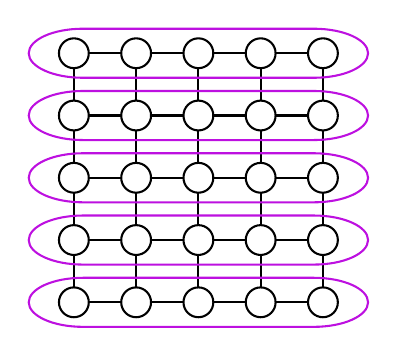
\begin{tikzpicture}[x=0.75pt,y=0.75pt,yscale=-1.5,xscale=1.5]
%uncomment if require: \path (0,115.140625); %set diagram left start at 0, and has height of 115.140625

%Shape: Grid [id:dp6398468642796289] 
\draw  [draw opacity=0][fill={rgb, 255:red, 255; green, 255; blue, 255 }  ,fill opacity=1 ] (289.5,18) -- (369.67,18) -- (369.67,98.5) -- (289.5,98.5) -- cycle ; \draw   (289.5,18) -- (289.5,98.5)(309.5,18) -- (309.5,98.5)(329.5,18) -- (329.5,98.5)(349.5,18) -- (349.5,98.5)(369.5,18) -- (369.5,98.5) ; \draw   (289.5,18) -- (369.67,18)(289.5,38) -- (369.67,38)(289.5,58) -- (369.67,58)(289.5,78) -- (369.67,78)(289.5,98) -- (369.67,98) ; \draw    ;
%Shape: Circle [id:dp45979430813709987] 
\draw  [fill={rgb, 255:red, 255; green, 255; blue, 255 }  ,fill opacity=1 ] (284.71,98) .. controls (284.71,95.35) and (286.85,93.21) .. (289.5,93.21) .. controls (292.15,93.21) and (294.29,95.35) .. (294.29,98) .. controls (294.29,100.65) and (292.15,102.79) .. (289.5,102.79) .. controls (286.85,102.79) and (284.71,100.65) .. (284.71,98) -- cycle ;
%Shape: Circle [id:dp6798408592338965] 
\draw  [fill={rgb, 255:red, 255; green, 255; blue, 255 }  ,fill opacity=1 ] (304.71,98) .. controls (304.71,95.35) and (306.85,93.21) .. (309.5,93.21) .. controls (312.15,93.21) and (314.29,95.35) .. (314.29,98) .. controls (314.29,100.65) and (312.15,102.79) .. (309.5,102.79) .. controls (306.85,102.79) and (304.71,100.65) .. (304.71,98) -- cycle ;
%Shape: Circle [id:dp43915410890453344] 
\draw  [fill={rgb, 255:red, 255; green, 255; blue, 255 }  ,fill opacity=1 ] (324.71,98) .. controls (324.71,95.35) and (326.85,93.21) .. (329.5,93.21) .. controls (332.15,93.21) and (334.29,95.35) .. (334.29,98) .. controls (334.29,100.65) and (332.15,102.79) .. (329.5,102.79) .. controls (326.85,102.79) and (324.71,100.65) .. (324.71,98) -- cycle ;
%Shape: Circle [id:dp6382986889249085] 
\draw  [fill={rgb, 255:red, 255; green, 255; blue, 255 }  ,fill opacity=1 ] (344.71,98) .. controls (344.71,95.35) and (346.85,93.21) .. (349.5,93.21) .. controls (352.15,93.21) and (354.29,95.35) .. (354.29,98) .. controls (354.29,100.65) and (352.15,102.79) .. (349.5,102.79) .. controls (346.85,102.79) and (344.71,100.65) .. (344.71,98) -- cycle ;
%Shape: Circle [id:dp3030458235296949] 
\draw  [fill={rgb, 255:red, 255; green, 255; blue, 255 }  ,fill opacity=1 ] (364.71,98) .. controls (364.71,95.35) and (366.85,93.21) .. (369.5,93.21) .. controls (372.15,93.21) and (374.29,95.35) .. (374.29,98) .. controls (374.29,100.65) and (372.15,102.79) .. (369.5,102.79) .. controls (366.85,102.79) and (364.71,100.65) .. (364.71,98) -- cycle ;
%Shape: Circle [id:dp24395857030962298] 
\draw  [fill={rgb, 255:red, 255; green, 255; blue, 255 }  ,fill opacity=1 ] (364.71,58) .. controls (364.71,55.35) and (366.85,53.21) .. (369.5,53.21) .. controls (372.15,53.21) and (374.29,55.35) .. (374.29,58) .. controls (374.29,60.65) and (372.15,62.79) .. (369.5,62.79) .. controls (366.85,62.79) and (364.71,60.65) .. (364.71,58) -- cycle ;
%Shape: Circle [id:dp691718311493239] 
\draw  [fill={rgb, 255:red, 255; green, 255; blue, 255 }  ,fill opacity=1 ] (364.71,78) .. controls (364.71,75.35) and (366.85,73.21) .. (369.5,73.21) .. controls (372.15,73.21) and (374.29,75.35) .. (374.29,78) .. controls (374.29,80.65) and (372.15,82.79) .. (369.5,82.79) .. controls (366.85,82.79) and (364.71,80.65) .. (364.71,78) -- cycle ;
%Shape: Circle [id:dp5314933096230425] 
\draw  [fill={rgb, 255:red, 255; green, 255; blue, 255 }  ,fill opacity=1 ] (344.71,78) .. controls (344.71,75.35) and (346.85,73.21) .. (349.5,73.21) .. controls (352.15,73.21) and (354.29,75.35) .. (354.29,78) .. controls (354.29,80.65) and (352.15,82.79) .. (349.5,82.79) .. controls (346.85,82.79) and (344.71,80.65) .. (344.71,78) -- cycle ;
%Shape: Circle [id:dp7377099421593283] 
\draw  [fill={rgb, 255:red, 255; green, 255; blue, 255 }  ,fill opacity=1 ] (324.71,78) .. controls (324.71,75.35) and (326.85,73.21) .. (329.5,73.21) .. controls (332.15,73.21) and (334.29,75.35) .. (334.29,78) .. controls (334.29,80.65) and (332.15,82.79) .. (329.5,82.79) .. controls (326.85,82.79) and (324.71,80.65) .. (324.71,78) -- cycle ;
%Shape: Circle [id:dp7015973959615016] 
\draw  [fill={rgb, 255:red, 255; green, 255; blue, 255 }  ,fill opacity=1 ] (304.71,78) .. controls (304.71,75.35) and (306.85,73.21) .. (309.5,73.21) .. controls (312.15,73.21) and (314.29,75.35) .. (314.29,78) .. controls (314.29,80.65) and (312.15,82.79) .. (309.5,82.79) .. controls (306.85,82.79) and (304.71,80.65) .. (304.71,78) -- cycle ;
%Shape: Circle [id:dp8830892952742624] 
\draw  [fill={rgb, 255:red, 255; green, 255; blue, 255 }  ,fill opacity=1 ] (284.71,78) .. controls (284.71,75.35) and (286.85,73.21) .. (289.5,73.21) .. controls (292.15,73.21) and (294.29,75.35) .. (294.29,78) .. controls (294.29,80.65) and (292.15,82.79) .. (289.5,82.79) .. controls (286.85,82.79) and (284.71,80.65) .. (284.71,78) -- cycle ;
%Shape: Circle [id:dp49879708058280725] 
\draw  [fill={rgb, 255:red, 255; green, 255; blue, 255 }  ,fill opacity=1 ] (284.71,58) .. controls (284.71,55.35) and (286.85,53.21) .. (289.5,53.21) .. controls (292.15,53.21) and (294.29,55.35) .. (294.29,58) .. controls (294.29,60.65) and (292.15,62.79) .. (289.5,62.79) .. controls (286.85,62.79) and (284.71,60.65) .. (284.71,58) -- cycle ;
%Shape: Circle [id:dp6127849824192515] 
\draw  [fill={rgb, 255:red, 255; green, 255; blue, 255 }  ,fill opacity=1 ] (304.71,58) .. controls (304.71,55.35) and (306.85,53.21) .. (309.5,53.21) .. controls (312.15,53.21) and (314.29,55.35) .. (314.29,58) .. controls (314.29,60.65) and (312.15,62.79) .. (309.5,62.79) .. controls (306.85,62.79) and (304.71,60.65) .. (304.71,58) -- cycle ;
%Shape: Circle [id:dp9331513706368058] 
\draw  [fill={rgb, 255:red, 255; green, 255; blue, 255 }  ,fill opacity=1 ] (324.71,58) .. controls (324.71,55.35) and (326.85,53.21) .. (329.5,53.21) .. controls (332.15,53.21) and (334.29,55.35) .. (334.29,58) .. controls (334.29,60.65) and (332.15,62.79) .. (329.5,62.79) .. controls (326.85,62.79) and (324.71,60.65) .. (324.71,58) -- cycle ;
%Shape: Circle [id:dp05112749299395425] 
\draw  [fill={rgb, 255:red, 255; green, 255; blue, 255 }  ,fill opacity=1 ] (344.71,58) .. controls (344.71,55.35) and (346.85,53.21) .. (349.5,53.21) .. controls (352.15,53.21) and (354.29,55.35) .. (354.29,58) .. controls (354.29,60.65) and (352.15,62.79) .. (349.5,62.79) .. controls (346.85,62.79) and (344.71,60.65) .. (344.71,58) -- cycle ;
%Shape: Circle [id:dp956420909230951] 
\draw  [fill={rgb, 255:red, 255; green, 255; blue, 255 }  ,fill opacity=1 ] (284.71,38) .. controls (284.71,35.35) and (286.85,33.21) .. (289.5,33.21) .. controls (292.15,33.21) and (294.29,35.35) .. (294.29,38) .. controls (294.29,40.65) and (292.15,42.79) .. (289.5,42.79) .. controls (286.85,42.79) and (284.71,40.65) .. (284.71,38) -- cycle ;
%Shape: Circle [id:dp8028524165446269] 
\draw  [fill={rgb, 255:red, 255; green, 255; blue, 255 }  ,fill opacity=1 ] (304.71,38) .. controls (304.71,35.35) and (306.85,33.21) .. (309.5,33.21) .. controls (312.15,33.21) and (314.29,35.35) .. (314.29,38) .. controls (314.29,40.65) and (312.15,42.79) .. (309.5,42.79) .. controls (306.85,42.79) and (304.71,40.65) .. (304.71,38) -- cycle ;
%Shape: Circle [id:dp46008411636229773] 
\draw  [fill={rgb, 255:red, 255; green, 255; blue, 255 }  ,fill opacity=1 ] (324.71,38) .. controls (324.71,35.35) and (326.85,33.21) .. (329.5,33.21) .. controls (332.15,33.21) and (334.29,35.35) .. (334.29,38) .. controls (334.29,40.65) and (332.15,42.79) .. (329.5,42.79) .. controls (326.85,42.79) and (324.71,40.65) .. (324.71,38) -- cycle ;
%Shape: Circle [id:dp5091438563989834] 
\draw  [fill={rgb, 255:red, 255; green, 255; blue, 255 }  ,fill opacity=1 ] (344.71,38) .. controls (344.71,35.35) and (346.85,33.21) .. (349.5,33.21) .. controls (352.15,33.21) and (354.29,35.35) .. (354.29,38) .. controls (354.29,40.65) and (352.15,42.79) .. (349.5,42.79) .. controls (346.85,42.79) and (344.71,40.65) .. (344.71,38) -- cycle ;
%Shape: Circle [id:dp2971421161467478] 
\draw  [fill={rgb, 255:red, 255; green, 255; blue, 255 }  ,fill opacity=1 ] (364.71,38) .. controls (364.71,35.35) and (366.85,33.21) .. (369.5,33.21) .. controls (372.15,33.21) and (374.29,35.35) .. (374.29,38) .. controls (374.29,40.65) and (372.15,42.79) .. (369.5,42.79) .. controls (366.85,42.79) and (364.71,40.65) .. (364.71,38) -- cycle ;
%Shape: Circle [id:dp7925033591002817] 
\draw  [fill={rgb, 255:red, 255; green, 255; blue, 255 }  ,fill opacity=1 ] (284.71,18) .. controls (284.71,15.35) and (286.85,13.21) .. (289.5,13.21) .. controls (292.15,13.21) and (294.29,15.35) .. (294.29,18) .. controls (294.29,20.65) and (292.15,22.79) .. (289.5,22.79) .. controls (286.85,22.79) and (284.71,20.65) .. (284.71,18) -- cycle ;
%Shape: Circle [id:dp136092262412969] 
\draw  [fill={rgb, 255:red, 255; green, 255; blue, 255 }  ,fill opacity=1 ] (304.71,18) .. controls (304.71,15.35) and (306.85,13.21) .. (309.5,13.21) .. controls (312.15,13.21) and (314.29,15.35) .. (314.29,18) .. controls (314.29,20.65) and (312.15,22.79) .. (309.5,22.79) .. controls (306.85,22.79) and (304.71,20.65) .. (304.71,18) -- cycle ;
%Shape: Circle [id:dp6893173867140368] 
\draw  [fill={rgb, 255:red, 255; green, 255; blue, 255 }  ,fill opacity=1 ] (324.71,18) .. controls (324.71,15.35) and (326.85,13.21) .. (329.5,13.21) .. controls (332.15,13.21) and (334.29,15.35) .. (334.29,18) .. controls (334.29,20.65) and (332.15,22.79) .. (329.5,22.79) .. controls (326.85,22.79) and (324.71,20.65) .. (324.71,18) -- cycle ;
%Shape: Circle [id:dp7052505194059135] 
\draw  [fill={rgb, 255:red, 255; green, 255; blue, 255 }  ,fill opacity=1 ] (344.71,18) .. controls (344.71,15.35) and (346.85,13.21) .. (349.5,13.21) .. controls (352.15,13.21) and (354.29,15.35) .. (354.29,18) .. controls (354.29,20.65) and (352.15,22.79) .. (349.5,22.79) .. controls (346.85,22.79) and (344.71,20.65) .. (344.71,18) -- cycle ;
%Shape: Circle [id:dp9728302946154153] 
\draw  [fill={rgb, 255:red, 255; green, 255; blue, 255 }  ,fill opacity=1 ] (364.71,18) .. controls (364.71,15.35) and (366.85,13.21) .. (369.5,13.21) .. controls (372.15,13.21) and (374.29,15.35) .. (374.29,18) .. controls (374.29,20.65) and (372.15,22.79) .. (369.5,22.79) .. controls (366.85,22.79) and (364.71,20.65) .. (364.71,18) -- cycle ;
%Flowchart: Terminator [id:dp402502914211049] 
\draw  [color={rgb, 255:red, 189; green, 16; blue, 224 }  ,draw opacity=1 ] (292.44,90.12) -- (366.56,90.12) .. controls (376.19,90.12) and (384,93.65) .. (384,98) .. controls (384,102.35) and (376.19,105.88) .. (366.56,105.88) -- (292.44,105.88) .. controls (282.81,105.88) and (275,102.35) .. (275,98) .. controls (275,93.65) and (282.81,90.12) .. (292.44,90.12) -- cycle ;
%Flowchart: Terminator [id:dp9672502771080671] 
\draw  [color={rgb, 255:red, 189; green, 16; blue, 224 }  ,draw opacity=1 ] (292.44,70.12) -- (366.56,70.12) .. controls (376.19,70.12) and (384,73.65) .. (384,78) .. controls (384,82.35) and (376.19,85.88) .. (366.56,85.88) -- (292.44,85.88) .. controls (282.81,85.88) and (275,82.35) .. (275,78) .. controls (275,73.65) and (282.81,70.12) .. (292.44,70.12) -- cycle ;
%Flowchart: Terminator [id:dp22570093409758574] 
\draw  [color={rgb, 255:red, 189; green, 16; blue, 224 }  ,draw opacity=1 ] (292.44,50.12) -- (366.56,50.12) .. controls (376.19,50.12) and (384,53.65) .. (384,58) .. controls (384,62.35) and (376.19,65.88) .. (366.56,65.88) -- (292.44,65.88) .. controls (282.81,65.88) and (275,62.35) .. (275,58) .. controls (275,53.65) and (282.81,50.12) .. (292.44,50.12) -- cycle ;
%Flowchart: Terminator [id:dp6938195823539697] 
\draw  [color={rgb, 255:red, 189; green, 16; blue, 224 }  ,draw opacity=1 ] (292.44,30.12) -- (366.56,30.12) .. controls (376.19,30.12) and (384,33.65) .. (384,38) .. controls (384,42.35) and (376.19,45.88) .. (366.56,45.88) -- (292.44,45.88) .. controls (282.81,45.88) and (275,42.35) .. (275,38) .. controls (275,33.65) and (282.81,30.12) .. (292.44,30.12) -- cycle ;
%Flowchart: Terminator [id:dp5985280356267675] 
\draw  [color={rgb, 255:red, 189; green, 16; blue, 224 }  ,draw opacity=1 ] (292.44,10.12) -- (366.56,10.12) .. controls (376.19,10.12) and (384,13.65) .. (384,18) .. controls (384,22.35) and (376.19,25.88) .. (366.56,25.88) -- (292.44,25.88) .. controls (282.81,25.88) and (275,22.35) .. (275,18) .. controls (275,13.65) and (282.81,10.12) .. (292.44,10.12) -- cycle ;

\end{tikzpicture}

	\end{center}
	\caption{horizontal splitting}
\end{figure}

\begin{figure}[H]
	\begin{center}
		\tikzset{every picture/.style={line width=0.75pt}} %set default line width to 0.75pt        

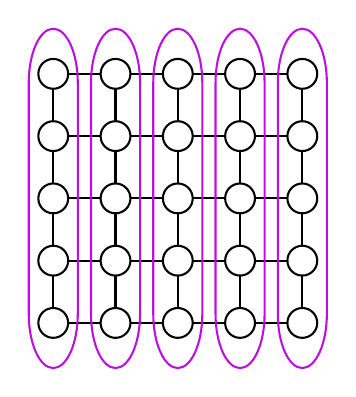
\begin{tikzpicture}[x=0.75pt,y=0.75pt,yscale=-1.5,xscale=1.5]
%uncomment if require: \path (0,130); %set diagram left start at 0, and has height of 130

%Shape: Grid [id:dp7399042803862277] 
\draw  [draw opacity=0][fill={rgb, 255:red, 255; green, 255; blue, 255 }  ,fill opacity=1 ] (369.5,25) -- (369.5,105.17) -- (289,105.17) -- (289,25) -- cycle ; \draw   (369.5,25) -- (289,25)(369.5,45) -- (289,45)(369.5,65) -- (289,65)(369.5,85) -- (289,85)(369.5,105) -- (289,105) ; \draw   (369.5,25) -- (369.5,105.17)(349.5,25) -- (349.5,105.17)(329.5,25) -- (329.5,105.17)(309.5,25) -- (309.5,105.17)(289.5,25) -- (289.5,105.17) ; \draw    ;
%Shape: Circle [id:dp8651637723303116] 
\draw  [fill={rgb, 255:red, 255; green, 255; blue, 255 }  ,fill opacity=1 ] (289.5,20.21) .. controls (292.15,20.21) and (294.29,22.35) .. (294.29,25) .. controls (294.29,27.65) and (292.15,29.79) .. (289.5,29.79) .. controls (286.85,29.79) and (284.71,27.65) .. (284.71,25) .. controls (284.71,22.35) and (286.85,20.21) .. (289.5,20.21) -- cycle ;
%Shape: Circle [id:dp9652078854977582] 
\draw  [fill={rgb, 255:red, 255; green, 255; blue, 255 }  ,fill opacity=1 ] (289.5,40.21) .. controls (292.15,40.21) and (294.29,42.35) .. (294.29,45) .. controls (294.29,47.65) and (292.15,49.79) .. (289.5,49.79) .. controls (286.85,49.79) and (284.71,47.65) .. (284.71,45) .. controls (284.71,42.35) and (286.85,40.21) .. (289.5,40.21) -- cycle ;
%Shape: Circle [id:dp1728749303967967] 
\draw  [fill={rgb, 255:red, 255; green, 255; blue, 255 }  ,fill opacity=1 ] (289.5,60.21) .. controls (292.15,60.21) and (294.29,62.35) .. (294.29,65) .. controls (294.29,67.65) and (292.15,69.79) .. (289.5,69.79) .. controls (286.85,69.79) and (284.71,67.65) .. (284.71,65) .. controls (284.71,62.35) and (286.85,60.21) .. (289.5,60.21) -- cycle ;
%Shape: Circle [id:dp23036347408038615] 
\draw  [fill={rgb, 255:red, 255; green, 255; blue, 255 }  ,fill opacity=1 ] (289.5,80.21) .. controls (292.15,80.21) and (294.29,82.35) .. (294.29,85) .. controls (294.29,87.65) and (292.15,89.79) .. (289.5,89.79) .. controls (286.85,89.79) and (284.71,87.65) .. (284.71,85) .. controls (284.71,82.35) and (286.85,80.21) .. (289.5,80.21) -- cycle ;
%Shape: Circle [id:dp44967083895831417] 
\draw  [fill={rgb, 255:red, 255; green, 255; blue, 255 }  ,fill opacity=1 ] (289.5,100.21) .. controls (292.15,100.21) and (294.29,102.35) .. (294.29,105) .. controls (294.29,107.65) and (292.15,109.79) .. (289.5,109.79) .. controls (286.85,109.79) and (284.71,107.65) .. (284.71,105) .. controls (284.71,102.35) and (286.85,100.21) .. (289.5,100.21) -- cycle ;
%Shape: Circle [id:dp9315039699787822] 
\draw  [fill={rgb, 255:red, 255; green, 255; blue, 255 }  ,fill opacity=1 ] (329.5,100.21) .. controls (332.15,100.21) and (334.29,102.35) .. (334.29,105) .. controls (334.29,107.65) and (332.15,109.79) .. (329.5,109.79) .. controls (326.85,109.79) and (324.71,107.65) .. (324.71,105) .. controls (324.71,102.35) and (326.85,100.21) .. (329.5,100.21) -- cycle ;
%Shape: Circle [id:dp5121103666957594] 
\draw  [fill={rgb, 255:red, 255; green, 255; blue, 255 }  ,fill opacity=1 ] (309.5,100.21) .. controls (312.15,100.21) and (314.29,102.35) .. (314.29,105) .. controls (314.29,107.65) and (312.15,109.79) .. (309.5,109.79) .. controls (306.85,109.79) and (304.71,107.65) .. (304.71,105) .. controls (304.71,102.35) and (306.85,100.21) .. (309.5,100.21) -- cycle ;
%Shape: Circle [id:dp4801713337694038] 
\draw  [fill={rgb, 255:red, 255; green, 255; blue, 255 }  ,fill opacity=1 ] (309.5,80.21) .. controls (312.15,80.21) and (314.29,82.35) .. (314.29,85) .. controls (314.29,87.65) and (312.15,89.79) .. (309.5,89.79) .. controls (306.85,89.79) and (304.71,87.65) .. (304.71,85) .. controls (304.71,82.35) and (306.85,80.21) .. (309.5,80.21) -- cycle ;
%Shape: Circle [id:dp12535689486360901] 
\draw  [fill={rgb, 255:red, 255; green, 255; blue, 255 }  ,fill opacity=1 ] (309.5,60.21) .. controls (312.15,60.21) and (314.29,62.35) .. (314.29,65) .. controls (314.29,67.65) and (312.15,69.79) .. (309.5,69.79) .. controls (306.85,69.79) and (304.71,67.65) .. (304.71,65) .. controls (304.71,62.35) and (306.85,60.21) .. (309.5,60.21) -- cycle ;
%Shape: Circle [id:dp46320678872772225] 
\draw  [fill={rgb, 255:red, 255; green, 255; blue, 255 }  ,fill opacity=1 ] (309.5,40.21) .. controls (312.15,40.21) and (314.29,42.35) .. (314.29,45) .. controls (314.29,47.65) and (312.15,49.79) .. (309.5,49.79) .. controls (306.85,49.79) and (304.71,47.65) .. (304.71,45) .. controls (304.71,42.35) and (306.85,40.21) .. (309.5,40.21) -- cycle ;
%Shape: Circle [id:dp6043516156300452] 
\draw  [fill={rgb, 255:red, 255; green, 255; blue, 255 }  ,fill opacity=1 ] (309.5,20.21) .. controls (312.15,20.21) and (314.29,22.35) .. (314.29,25) .. controls (314.29,27.65) and (312.15,29.79) .. (309.5,29.79) .. controls (306.85,29.79) and (304.71,27.65) .. (304.71,25) .. controls (304.71,22.35) and (306.85,20.21) .. (309.5,20.21) -- cycle ;
%Shape: Circle [id:dp6332387096370653] 
\draw  [fill={rgb, 255:red, 255; green, 255; blue, 255 }  ,fill opacity=1 ] (329.5,20.21) .. controls (332.15,20.21) and (334.29,22.35) .. (334.29,25) .. controls (334.29,27.65) and (332.15,29.79) .. (329.5,29.79) .. controls (326.85,29.79) and (324.71,27.65) .. (324.71,25) .. controls (324.71,22.35) and (326.85,20.21) .. (329.5,20.21) -- cycle ;
%Shape: Circle [id:dp055019880981398206] 
\draw  [fill={rgb, 255:red, 255; green, 255; blue, 255 }  ,fill opacity=1 ] (329.5,40.21) .. controls (332.15,40.21) and (334.29,42.35) .. (334.29,45) .. controls (334.29,47.65) and (332.15,49.79) .. (329.5,49.79) .. controls (326.85,49.79) and (324.71,47.65) .. (324.71,45) .. controls (324.71,42.35) and (326.85,40.21) .. (329.5,40.21) -- cycle ;
%Shape: Circle [id:dp8512639356233513] 
\draw  [fill={rgb, 255:red, 255; green, 255; blue, 255 }  ,fill opacity=1 ] (329.5,60.21) .. controls (332.15,60.21) and (334.29,62.35) .. (334.29,65) .. controls (334.29,67.65) and (332.15,69.79) .. (329.5,69.79) .. controls (326.85,69.79) and (324.71,67.65) .. (324.71,65) .. controls (324.71,62.35) and (326.85,60.21) .. (329.5,60.21) -- cycle ;
%Shape: Circle [id:dp6205062014645637] 
\draw  [fill={rgb, 255:red, 255; green, 255; blue, 255 }  ,fill opacity=1 ] (329.5,80.21) .. controls (332.15,80.21) and (334.29,82.35) .. (334.29,85) .. controls (334.29,87.65) and (332.15,89.79) .. (329.5,89.79) .. controls (326.85,89.79) and (324.71,87.65) .. (324.71,85) .. controls (324.71,82.35) and (326.85,80.21) .. (329.5,80.21) -- cycle ;
%Shape: Circle [id:dp222923337548673] 
\draw  [fill={rgb, 255:red, 255; green, 255; blue, 255 }  ,fill opacity=1 ] (349.5,20.21) .. controls (352.15,20.21) and (354.29,22.35) .. (354.29,25) .. controls (354.29,27.65) and (352.15,29.79) .. (349.5,29.79) .. controls (346.85,29.79) and (344.71,27.65) .. (344.71,25) .. controls (344.71,22.35) and (346.85,20.21) .. (349.5,20.21) -- cycle ;
%Shape: Circle [id:dp6018140604006843] 
\draw  [fill={rgb, 255:red, 255; green, 255; blue, 255 }  ,fill opacity=1 ] (349.5,40.21) .. controls (352.15,40.21) and (354.29,42.35) .. (354.29,45) .. controls (354.29,47.65) and (352.15,49.79) .. (349.5,49.79) .. controls (346.85,49.79) and (344.71,47.65) .. (344.71,45) .. controls (344.71,42.35) and (346.85,40.21) .. (349.5,40.21) -- cycle ;
%Shape: Circle [id:dp6348042495140271] 
\draw  [fill={rgb, 255:red, 255; green, 255; blue, 255 }  ,fill opacity=1 ] (349.5,60.21) .. controls (352.15,60.21) and (354.29,62.35) .. (354.29,65) .. controls (354.29,67.65) and (352.15,69.79) .. (349.5,69.79) .. controls (346.85,69.79) and (344.71,67.65) .. (344.71,65) .. controls (344.71,62.35) and (346.85,60.21) .. (349.5,60.21) -- cycle ;
%Shape: Circle [id:dp9647261865514132] 
\draw  [fill={rgb, 255:red, 255; green, 255; blue, 255 }  ,fill opacity=1 ] (349.5,80.21) .. controls (352.15,80.21) and (354.29,82.35) .. (354.29,85) .. controls (354.29,87.65) and (352.15,89.79) .. (349.5,89.79) .. controls (346.85,89.79) and (344.71,87.65) .. (344.71,85) .. controls (344.71,82.35) and (346.85,80.21) .. (349.5,80.21) -- cycle ;
%Shape: Circle [id:dp5724526378156161] 
\draw  [fill={rgb, 255:red, 255; green, 255; blue, 255 }  ,fill opacity=1 ] (349.5,100.21) .. controls (352.15,100.21) and (354.29,102.35) .. (354.29,105) .. controls (354.29,107.65) and (352.15,109.79) .. (349.5,109.79) .. controls (346.85,109.79) and (344.71,107.65) .. (344.71,105) .. controls (344.71,102.35) and (346.85,100.21) .. (349.5,100.21) -- cycle ;
%Shape: Circle [id:dp25061370635376257] 
\draw  [fill={rgb, 255:red, 255; green, 255; blue, 255 }  ,fill opacity=1 ] (369.5,20.21) .. controls (372.15,20.21) and (374.29,22.35) .. (374.29,25) .. controls (374.29,27.65) and (372.15,29.79) .. (369.5,29.79) .. controls (366.85,29.79) and (364.71,27.65) .. (364.71,25) .. controls (364.71,22.35) and (366.85,20.21) .. (369.5,20.21) -- cycle ;
%Shape: Circle [id:dp8340204987440425] 
\draw  [fill={rgb, 255:red, 255; green, 255; blue, 255 }  ,fill opacity=1 ] (369.5,40.21) .. controls (372.15,40.21) and (374.29,42.35) .. (374.29,45) .. controls (374.29,47.65) and (372.15,49.79) .. (369.5,49.79) .. controls (366.85,49.79) and (364.71,47.65) .. (364.71,45) .. controls (364.71,42.35) and (366.85,40.21) .. (369.5,40.21) -- cycle ;
%Shape: Circle [id:dp5677261375761635] 
\draw  [fill={rgb, 255:red, 255; green, 255; blue, 255 }  ,fill opacity=1 ] (369.5,60.21) .. controls (372.15,60.21) and (374.29,62.35) .. (374.29,65) .. controls (374.29,67.65) and (372.15,69.79) .. (369.5,69.79) .. controls (366.85,69.79) and (364.71,67.65) .. (364.71,65) .. controls (364.71,62.35) and (366.85,60.21) .. (369.5,60.21) -- cycle ;
%Shape: Circle [id:dp25189376094363247] 
\draw  [fill={rgb, 255:red, 255; green, 255; blue, 255 }  ,fill opacity=1 ] (369.5,80.21) .. controls (372.15,80.21) and (374.29,82.35) .. (374.29,85) .. controls (374.29,87.65) and (372.15,89.79) .. (369.5,89.79) .. controls (366.85,89.79) and (364.71,87.65) .. (364.71,85) .. controls (364.71,82.35) and (366.85,80.21) .. (369.5,80.21) -- cycle ;
%Shape: Circle [id:dp6141487714233882] 
\draw  [fill={rgb, 255:red, 255; green, 255; blue, 255 }  ,fill opacity=1 ] (369.5,100.21) .. controls (372.15,100.21) and (374.29,102.35) .. (374.29,105) .. controls (374.29,107.65) and (372.15,109.79) .. (369.5,109.79) .. controls (366.85,109.79) and (364.71,107.65) .. (364.71,105) .. controls (364.71,102.35) and (366.85,100.21) .. (369.5,100.21) -- cycle ;
%Flowchart: Terminator [id:dp5771267457316103] 
\draw  [color={rgb, 255:red, 189; green, 16; blue, 224 }  ,draw opacity=1 ] (297.38,27.94) -- (297.38,102.06) .. controls (297.38,111.69) and (293.85,119.5) .. (289.5,119.5) .. controls (285.15,119.5) and (281.62,111.69) .. (281.62,102.06) -- (281.62,27.94) .. controls (281.62,18.31) and (285.15,10.5) .. (289.5,10.5) .. controls (293.85,10.5) and (297.38,18.31) .. (297.38,27.94) -- cycle ;
%Flowchart: Terminator [id:dp1699164006075664] 
\draw  [color={rgb, 255:red, 189; green, 16; blue, 224 }  ,draw opacity=1 ] (317.38,27.94) -- (317.38,102.06) .. controls (317.38,111.69) and (313.85,119.5) .. (309.5,119.5) .. controls (305.15,119.5) and (301.62,111.69) .. (301.62,102.06) -- (301.62,27.94) .. controls (301.62,18.31) and (305.15,10.5) .. (309.5,10.5) .. controls (313.85,10.5) and (317.38,18.31) .. (317.38,27.94) -- cycle ;
%Flowchart: Terminator [id:dp4431975324978088] 
\draw  [color={rgb, 255:red, 189; green, 16; blue, 224 }  ,draw opacity=1 ] (337.38,27.94) -- (337.38,102.06) .. controls (337.38,111.69) and (333.85,119.5) .. (329.5,119.5) .. controls (325.15,119.5) and (321.62,111.69) .. (321.62,102.06) -- (321.62,27.94) .. controls (321.62,18.31) and (325.15,10.5) .. (329.5,10.5) .. controls (333.85,10.5) and (337.38,18.31) .. (337.38,27.94) -- cycle ;
%Flowchart: Terminator [id:dp948813775073037] 
\draw  [color={rgb, 255:red, 189; green, 16; blue, 224 }  ,draw opacity=1 ] (357.38,27.94) -- (357.38,102.06) .. controls (357.38,111.69) and (353.85,119.5) .. (349.5,119.5) .. controls (345.15,119.5) and (341.62,111.69) .. (341.62,102.06) -- (341.62,27.94) .. controls (341.62,18.31) and (345.15,10.5) .. (349.5,10.5) .. controls (353.85,10.5) and (357.38,18.31) .. (357.38,27.94) -- cycle ;
%Flowchart: Terminator [id:dp22652637896563754] 
\draw  [color={rgb, 255:red, 189; green, 16; blue, 224 }  ,draw opacity=1 ] (377.38,27.94) -- (377.38,102.06) .. controls (377.38,111.69) and (373.85,119.5) .. (369.5,119.5) .. controls (365.15,119.5) and (361.62,111.69) .. (361.62,102.06) -- (361.62,27.94) .. controls (361.62,18.31) and (365.15,10.5) .. (369.5,10.5) .. controls (373.85,10.5) and (377.38,18.31) .. (377.38,27.94) -- cycle ;
\end{tikzpicture}

	\end{center}
	\caption{vertical splitting}
\end{figure}

Then there methods of Multi-Splitting with line-relaxation in two different directions. This method is called the Alternating-Direction-Method.

\subsection*{Gauss-Seidel and SOR Parallelization}
\label{sec:Gauss-Seidel and SOR Parallelization}

\begin{figure}[H]
	\begin{center}
		

\tikzset{every picture/.style={line width=0.75pt}} %set default line width to 0.75pt        

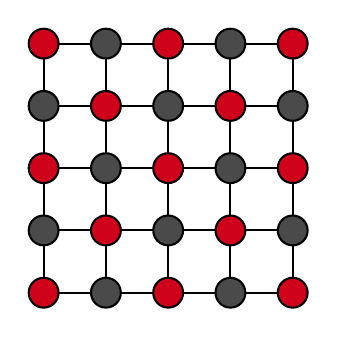
\begin{tikzpicture}[x=0.75pt,y=0.75pt,yscale=-1.5,xscale=1.5]
%uncomment if require: \path (0,222); %set diagram left start at 0, and has height of 222

%Shape: Grid [id:dp7509010194001084] 
\draw  [draw opacity=0][fill={rgb, 255:red, 255; green, 255; blue, 255 }  ,fill opacity=1 ] (289.5,76) -- (369.67,76) -- (369.67,156.5) -- (289.5,156.5) -- cycle ; \draw   (289.5,76) -- (289.5,156.5)(309.5,76) -- (309.5,156.5)(329.5,76) -- (329.5,156.5)(349.5,76) -- (349.5,156.5)(369.5,76) -- (369.5,156.5) ; \draw   (289.5,76) -- (369.67,76)(289.5,96) -- (369.67,96)(289.5,116) -- (369.67,116)(289.5,136) -- (369.67,136)(289.5,156) -- (369.67,156) ; \draw    ;
%Shape: Circle [id:dp6108755291859196] 
\draw  [fill={rgb, 255:red, 208; green, 2; blue, 27 }  ,fill opacity=1 ] (284.71,156) .. controls (284.71,153.35) and (286.85,151.21) .. (289.5,151.21) .. controls (292.15,151.21) and (294.29,153.35) .. (294.29,156) .. controls (294.29,158.65) and (292.15,160.79) .. (289.5,160.79) .. controls (286.85,160.79) and (284.71,158.65) .. (284.71,156) -- cycle ;
%Shape: Circle [id:dp4441687082516983] 
\draw  [fill={rgb, 255:red, 74; green, 74; blue, 74 }  ,fill opacity=1 ] (304.71,156) .. controls (304.71,153.35) and (306.85,151.21) .. (309.5,151.21) .. controls (312.15,151.21) and (314.29,153.35) .. (314.29,156) .. controls (314.29,158.65) and (312.15,160.79) .. (309.5,160.79) .. controls (306.85,160.79) and (304.71,158.65) .. (304.71,156) -- cycle ;
%Shape: Circle [id:dp6167896316379069] 
\draw  [fill={rgb, 255:red, 208; green, 2; blue, 27 }  ,fill opacity=1 ] (324.71,156) .. controls (324.71,153.35) and (326.85,151.21) .. (329.5,151.21) .. controls (332.15,151.21) and (334.29,153.35) .. (334.29,156) .. controls (334.29,158.65) and (332.15,160.79) .. (329.5,160.79) .. controls (326.85,160.79) and (324.71,158.65) .. (324.71,156) -- cycle ;
%Shape: Circle [id:dp6715236044117903] 
\draw  [fill={rgb, 255:red, 74; green, 74; blue, 74 }  ,fill opacity=1 ] (344.71,156) .. controls (344.71,153.35) and (346.85,151.21) .. (349.5,151.21) .. controls (352.15,151.21) and (354.29,153.35) .. (354.29,156) .. controls (354.29,158.65) and (352.15,160.79) .. (349.5,160.79) .. controls (346.85,160.79) and (344.71,158.65) .. (344.71,156) -- cycle ;
%Shape: Circle [id:dp06410493254248473] 
\draw  [fill={rgb, 255:red, 208; green, 2; blue, 27 }  ,fill opacity=1 ] (364.71,156) .. controls (364.71,153.35) and (366.85,151.21) .. (369.5,151.21) .. controls (372.15,151.21) and (374.29,153.35) .. (374.29,156) .. controls (374.29,158.65) and (372.15,160.79) .. (369.5,160.79) .. controls (366.85,160.79) and (364.71,158.65) .. (364.71,156) -- cycle ;
%Shape: Circle [id:dp6649764858783351] 
\draw  [fill={rgb, 255:red, 208; green, 2; blue, 27 }  ,fill opacity=1 ] (364.71,116) .. controls (364.71,113.35) and (366.85,111.21) .. (369.5,111.21) .. controls (372.15,111.21) and (374.29,113.35) .. (374.29,116) .. controls (374.29,118.65) and (372.15,120.79) .. (369.5,120.79) .. controls (366.85,120.79) and (364.71,118.65) .. (364.71,116) -- cycle ;
%Shape: Circle [id:dp9554900297815432] 
\draw  [fill={rgb, 255:red, 74; green, 74; blue, 74 }  ,fill opacity=1 ] (364.71,136) .. controls (364.71,133.35) and (366.85,131.21) .. (369.5,131.21) .. controls (372.15,131.21) and (374.29,133.35) .. (374.29,136) .. controls (374.29,138.65) and (372.15,140.79) .. (369.5,140.79) .. controls (366.85,140.79) and (364.71,138.65) .. (364.71,136) -- cycle ;
%Shape: Circle [id:dp37112581806137124] 
\draw  [fill={rgb, 255:red, 208; green, 2; blue, 27 }  ,fill opacity=1 ] (344.71,136) .. controls (344.71,133.35) and (346.85,131.21) .. (349.5,131.21) .. controls (352.15,131.21) and (354.29,133.35) .. (354.29,136) .. controls (354.29,138.65) and (352.15,140.79) .. (349.5,140.79) .. controls (346.85,140.79) and (344.71,138.65) .. (344.71,136) -- cycle ;
%Shape: Circle [id:dp06306680838602707] 
\draw  [fill={rgb, 255:red, 74; green, 74; blue, 74 }  ,fill opacity=1 ] (324.71,136) .. controls (324.71,133.35) and (326.85,131.21) .. (329.5,131.21) .. controls (332.15,131.21) and (334.29,133.35) .. (334.29,136) .. controls (334.29,138.65) and (332.15,140.79) .. (329.5,140.79) .. controls (326.85,140.79) and (324.71,138.65) .. (324.71,136) -- cycle ;
%Shape: Circle [id:dp9358022961380756] 
\draw  [fill={rgb, 255:red, 208; green, 2; blue, 27 }  ,fill opacity=1 ] (304.71,136) .. controls (304.71,133.35) and (306.85,131.21) .. (309.5,131.21) .. controls (312.15,131.21) and (314.29,133.35) .. (314.29,136) .. controls (314.29,138.65) and (312.15,140.79) .. (309.5,140.79) .. controls (306.85,140.79) and (304.71,138.65) .. (304.71,136) -- cycle ;
%Shape: Circle [id:dp9068520178890649] 
\draw  [fill={rgb, 255:red, 74; green, 74; blue, 74 }  ,fill opacity=1 ] (284.71,136) .. controls (284.71,133.35) and (286.85,131.21) .. (289.5,131.21) .. controls (292.15,131.21) and (294.29,133.35) .. (294.29,136) .. controls (294.29,138.65) and (292.15,140.79) .. (289.5,140.79) .. controls (286.85,140.79) and (284.71,138.65) .. (284.71,136) -- cycle ;
%Shape: Circle [id:dp8562155796812134] 
\draw  [fill={rgb, 255:red, 208; green, 2; blue, 27 }  ,fill opacity=1 ] (284.71,116) .. controls (284.71,113.35) and (286.85,111.21) .. (289.5,111.21) .. controls (292.15,111.21) and (294.29,113.35) .. (294.29,116) .. controls (294.29,118.65) and (292.15,120.79) .. (289.5,120.79) .. controls (286.85,120.79) and (284.71,118.65) .. (284.71,116) -- cycle ;
%Shape: Circle [id:dp2479839382803859] 
\draw  [fill={rgb, 255:red, 74; green, 74; blue, 74 }  ,fill opacity=1 ] (304.71,116) .. controls (304.71,113.35) and (306.85,111.21) .. (309.5,111.21) .. controls (312.15,111.21) and (314.29,113.35) .. (314.29,116) .. controls (314.29,118.65) and (312.15,120.79) .. (309.5,120.79) .. controls (306.85,120.79) and (304.71,118.65) .. (304.71,116) -- cycle ;
%Shape: Circle [id:dp8339992993489453] 
\draw  [fill={rgb, 255:red, 208; green, 2; blue, 27 }  ,fill opacity=1 ] (324.71,116) .. controls (324.71,113.35) and (326.85,111.21) .. (329.5,111.21) .. controls (332.15,111.21) and (334.29,113.35) .. (334.29,116) .. controls (334.29,118.65) and (332.15,120.79) .. (329.5,120.79) .. controls (326.85,120.79) and (324.71,118.65) .. (324.71,116) -- cycle ;
%Shape: Circle [id:dp29657132974437017] 
\draw  [fill={rgb, 255:red, 74; green, 74; blue, 74 }  ,fill opacity=1 ] (344.71,116) .. controls (344.71,113.35) and (346.85,111.21) .. (349.5,111.21) .. controls (352.15,111.21) and (354.29,113.35) .. (354.29,116) .. controls (354.29,118.65) and (352.15,120.79) .. (349.5,120.79) .. controls (346.85,120.79) and (344.71,118.65) .. (344.71,116) -- cycle ;
%Shape: Circle [id:dp4006844726389853] 
\draw  [fill={rgb, 255:red, 74; green, 74; blue, 74 }  ,fill opacity=1 ] (284.71,96) .. controls (284.71,93.35) and (286.85,91.21) .. (289.5,91.21) .. controls (292.15,91.21) and (294.29,93.35) .. (294.29,96) .. controls (294.29,98.65) and (292.15,100.79) .. (289.5,100.79) .. controls (286.85,100.79) and (284.71,98.65) .. (284.71,96) -- cycle ;
%Shape: Circle [id:dp2518725902881924] 
\draw  [fill={rgb, 255:red, 208; green, 2; blue, 27 }  ,fill opacity=1 ] (304.71,96) .. controls (304.71,93.35) and (306.85,91.21) .. (309.5,91.21) .. controls (312.15,91.21) and (314.29,93.35) .. (314.29,96) .. controls (314.29,98.65) and (312.15,100.79) .. (309.5,100.79) .. controls (306.85,100.79) and (304.71,98.65) .. (304.71,96) -- cycle ;
%Shape: Circle [id:dp9478829895408571] 
\draw  [fill={rgb, 255:red, 74; green, 74; blue, 74 }  ,fill opacity=1 ] (324.71,96) .. controls (324.71,93.35) and (326.85,91.21) .. (329.5,91.21) .. controls (332.15,91.21) and (334.29,93.35) .. (334.29,96) .. controls (334.29,98.65) and (332.15,100.79) .. (329.5,100.79) .. controls (326.85,100.79) and (324.71,98.65) .. (324.71,96) -- cycle ;
%Shape: Circle [id:dp5111042484735311] 
\draw  [fill={rgb, 255:red, 208; green, 2; blue, 27 }  ,fill opacity=1 ] (344.71,96) .. controls (344.71,93.35) and (346.85,91.21) .. (349.5,91.21) .. controls (352.15,91.21) and (354.29,93.35) .. (354.29,96) .. controls (354.29,98.65) and (352.15,100.79) .. (349.5,100.79) .. controls (346.85,100.79) and (344.71,98.65) .. (344.71,96) -- cycle ;
%Shape: Circle [id:dp08226041749176072] 
\draw  [fill={rgb, 255:red, 74; green, 74; blue, 74 }  ,fill opacity=1 ] (364.71,96) .. controls (364.71,93.35) and (366.85,91.21) .. (369.5,91.21) .. controls (372.15,91.21) and (374.29,93.35) .. (374.29,96) .. controls (374.29,98.65) and (372.15,100.79) .. (369.5,100.79) .. controls (366.85,100.79) and (364.71,98.65) .. (364.71,96) -- cycle ;
%Shape: Circle [id:dp6793036732090996] 
\draw  [fill={rgb, 255:red, 208; green, 2; blue, 27 }  ,fill opacity=1 ] (284.71,76) .. controls (284.71,73.35) and (286.85,71.21) .. (289.5,71.21) .. controls (292.15,71.21) and (294.29,73.35) .. (294.29,76) .. controls (294.29,78.65) and (292.15,80.79) .. (289.5,80.79) .. controls (286.85,80.79) and (284.71,78.65) .. (284.71,76) -- cycle ;
%Shape: Circle [id:dp4959600894339744] 
\draw  [fill={rgb, 255:red, 74; green, 74; blue, 74 }  ,fill opacity=1 ] (304.71,76) .. controls (304.71,73.35) and (306.85,71.21) .. (309.5,71.21) .. controls (312.15,71.21) and (314.29,73.35) .. (314.29,76) .. controls (314.29,78.65) and (312.15,80.79) .. (309.5,80.79) .. controls (306.85,80.79) and (304.71,78.65) .. (304.71,76) -- cycle ;
%Shape: Circle [id:dp9621563131775881] 
\draw  [fill={rgb, 255:red, 208; green, 2; blue, 27 }  ,fill opacity=1 ] (324.71,76) .. controls (324.71,73.35) and (326.85,71.21) .. (329.5,71.21) .. controls (332.15,71.21) and (334.29,73.35) .. (334.29,76) .. controls (334.29,78.65) and (332.15,80.79) .. (329.5,80.79) .. controls (326.85,80.79) and (324.71,78.65) .. (324.71,76) -- cycle ;
%Shape: Circle [id:dp06302816821338242] 
\draw  [fill={rgb, 255:red, 74; green, 74; blue, 74 }  ,fill opacity=1 ] (344.71,76) .. controls (344.71,73.35) and (346.85,71.21) .. (349.5,71.21) .. controls (352.15,71.21) and (354.29,73.35) .. (354.29,76) .. controls (354.29,78.65) and (352.15,80.79) .. (349.5,80.79) .. controls (346.85,80.79) and (344.71,78.65) .. (344.71,76) -- cycle ;
%Shape: Circle [id:dp40969700298757994] 
\draw  [fill={rgb, 255:red, 208; green, 2; blue, 27 }  ,fill opacity=1 ] (364.71,76) .. controls (364.71,73.35) and (366.85,71.21) .. (369.5,71.21) .. controls (372.15,71.21) and (374.29,73.35) .. (374.29,76) .. controls (374.29,78.65) and (372.15,80.79) .. (369.5,80.79) .. controls (366.85,80.79) and (364.71,78.65) .. (364.71,76) -- cycle ;

% Text Node
\draw (289.5,156) node [scale=1,color={rgb, 255:red, 255; green, 255; blue, 255 }  ,opacity=1 ] [align=left] {};
% Text Node
\draw (329.5,156) node [scale=1,color={rgb, 255:red, 255; green, 255; blue, 255 }  ,opacity=1 ] [align=left] {};
% Text Node
\draw (369.5,156) node [scale=1,color={rgb, 255:red, 255; green, 255; blue, 255 }  ,opacity=1 ] [align=left] {};
% Text Node
\draw (309.5,136) node [scale=1,color={rgb, 255:red, 255; green, 255; blue, 255 }  ,opacity=1 ] [align=left] {};
% Text Node
\draw (349.5,136) node [scale=1,color={rgb, 255:red, 255; green, 255; blue, 255 }  ,opacity=1 ] [align=left] {};
% Text Node
\draw (289.5,116) node [scale=1,color={rgb, 255:red, 255; green, 255; blue, 255 }  ,opacity=1 ] [align=left] {};
% Text Node
\draw (329.5,116) node [scale=1,color={rgb, 255:red, 255; green, 255; blue, 255 }  ,opacity=1 ] [align=left] {};
% Text Node
\draw (369.5,116) node [scale=1,color={rgb, 255:red, 255; green, 255; blue, 255 }  ,opacity=1 ] [align=left] {};
% Text Node
\draw (309.5,96) node [scale=1,color={rgb, 255:red, 255; green, 255; blue, 255 }  ,opacity=1 ] [align=left] {};
% Text Node
\draw (349.5,96) node [scale=1,color={rgb, 255:red, 255; green, 255; blue, 255 }  ,opacity=1 ] [align=left] {};
% Text Node
\draw (289.5,76) node [scale=1,color={rgb, 255:red, 255; green, 255; blue, 255 }  ,opacity=1 ] [align=left] {};
% Text Node
\draw (329.5,76) node [scale=1,color={rgb, 255:red, 255; green, 255; blue, 255 }  ,opacity=1 ] [align=left] {};
% Text Node
\draw (369.5,76) node [scale=1,color={rgb, 255:red, 255; green, 255; blue, 255 }  ,opacity=1 ] [align=left] {};
% Text Node
\draw (309.5,156) node [scale=1,color={rgb, 255:red, 255; green, 255; blue, 255 }  ,opacity=1 ] [align=left] {};
% Text Node
\draw (349.5,156) node [scale=1,color={rgb, 255:red, 255; green, 255; blue, 255 }  ,opacity=1 ] [align=left] {};
% Text Node
\draw (289.5,136) node [scale=1,color={rgb, 255:red, 255; green, 255; blue, 255 }  ,opacity=1 ] [align=left] {};
% Text Node
\draw (329.5,136) node [scale=1,color={rgb, 255:red, 255; green, 255; blue, 255 }  ,opacity=1 ] [align=left] {};
% Text Node
\draw (369.5,136) node [scale=1,color={rgb, 255:red, 255; green, 255; blue, 255 }  ,opacity=1 ] [align=left] {};
% Text Node
\draw (309.5,116) node [scale=1,color={rgb, 255:red, 255; green, 255; blue, 255 }  ,opacity=1 ] [align=left] {};
% Text Node
\draw (349.5,116) node [scale=1,color={rgb, 255:red, 255; green, 255; blue, 255 }  ,opacity=1 ] [align=left] {};
% Text Node
\draw (289.5,96) node [scale=1,color={rgb, 255:red, 255; green, 255; blue, 255 }  ,opacity=1 ] [align=left] {};
% Text Node
\draw (329.5,96) node [scale=1,color={rgb, 255:red, 255; green, 255; blue, 255 }  ,opacity=1 ] [align=left] {};
% Text Node
\draw (369.5,96) node [scale=1,color={rgb, 255:red, 255; green, 255; blue, 255 }  ,opacity=1 ] [align=left] {};
% Text Node
\draw (309.5,76) node [scale=1,color={rgb, 255:red, 255; green, 255; blue, 255 }  ,opacity=1 ] [align=left] {};
% Text Node
\draw (349.5,76) node [scale=1,color={rgb, 255:red, 255; green, 255; blue, 255 }  ,opacity=1 ] [align=left] {};


\end{tikzpicture}

	\end{center}
	\caption{vertical splitting}
\end{figure}

Resulting matrix
\[
A = \begin{bmatrix}
\begin{matrix}
-4\\
& \ddots \\
&& -4
\end{matrix}
&
\begin{matrix}
	E
\end{matrix}
\\
\begin{matrix}
	E^{T}
\end{matrix}
&
\begin{matrix}
-4\\
& \ddots \\
&& -4
\end{matrix}
\end{bmatrix}
,\] 
where $E$ describes the dependencies between the red and black nodes.
After simplifying, this can be denoted by
\[
A = \begin{pmatrix}
	D_{\text{red}} & E \\
	E^{T} & D_{\text{black}}
\end{pmatrix}
.\] 
With
\[
	(D-L) x^{k+1} = Ux^{k}+b \quad \text{ and } \quad (D-L) = \begin{pmatrix}
	D_{\text{red}} & E \\
	E^{T} & D_{\text{black}}
	\end{pmatrix}
\] 
we get
\[
\begin{pmatrix}
	D_{\text{red}} & 0 \\
	E^{T} & D_{\text{black}}
\end{pmatrix}
\begin{pmatrix}
x^{k+1}_{\text{red}} \\
x^{k+1}_{\text{black}}
\end{pmatrix}
=
\begin{pmatrix}
	0 & -E \\
	0 & 0
\end{pmatrix}
\begin{pmatrix}
x^{k}_{\text{red}} \\
x^{k}_{\text{black}}
\end{pmatrix}
+
\begin{pmatrix}
b_{\text{red}} \\
b_{\text{black}}
\end{pmatrix}
.\] 
So we basically have abstracted the updated step into two parts, which can be parallelized:
\begin{align*}
	D_{\text{red}}x_{\text{red}}^{k+1} &= -E x_{\text{black}}^{k} + b_{\text{red}} \\
	D_{\text{black}}x_{\text{black}}^{k+1} + E^{T} x_{\text{red}}^{k+1} &= b_{\text{black}}
\end{align*}
